\graphicspath{ {./pics/Matrix/} }

\section*{Matrix}
\hspace{1cm}
\rowcolors{1}{blue!10}{white}
\begin{tabular}{|l|}
 	\hline
	 np.array(object, dtype=None, *, copy=True, order="K", subok=False, ndmin=0) ndarray
	 \\ np.arange([start,] stop[, step,]dtype=None) ndarray
	 \\ np.asarray(a, dtype=None, order=None, *, like=None) ndarray
	 \\ np.copy(a, order="K", subok=False) ndarray
	 \\ np.empty(shape, dtype=float, order="C") int ndarray
	 \\ np.empty\_like(prototype, dtype=None, order="K", subok=True, shape=None) ndarray
	 \\ np.eye(N, M=None, k=0, dtype=<class "float">, order="C") ndarray
	 \\ np.full(shape, fill value, dtype=None, order="C") ndarray
	 \\ np.full like(a, fill value, dtype=None, order="K", subok=True, shape=None) ndarray
	 \\ np.fromfile(file, dtype=float, count=-1, sep=, offset=0) ndarray
	 \\ np.fromstring(string, dtype=float, count=-1, sep=) ndarray
	 \\ np.identity(n, dtype=None) ndarray
	 \\ np.linspace(start, stop, num=50, endpoint=True, retstep=False, dtype=None, axis=0) ndarray
	 \\ np.loadtxt(fname, dtype= $\langle$ class "float" $\rangle$ , comments="\#", delimiter=None, converters=None,
	 \\ skiprows=0,  usecols=None, unpack=False, ndmin=0, encoding="bytes", max rows=None) ndarray
	 \\ np.logspace(start, stop, num=50, endpoint=True, base=10.0, dtype=None, axis=0) ndarray
	 \\ np.meshgrid(*xi, copy=True, sparse=False, indexing="xy") ndarray
	 \\ np.ones(shape, dtype=None, order="C") ndarray
	 \\ np.ones like(a, dtype=None, order="K", subok=True, shape=None) ndarray
	 \\ np.random.randn(d0, d1, ...,dn) ndarray
	 \\ np.random.randint(low, high=None, size=None, dtype=int) ndarray
	 \\ np.zeros(shape, dtype=float, order="C") ndarray
	 \\ np.zeros like(a, dtype=None, order="K", subok=True, shape=None) ndarray
	\\\hline
\end{tabular}
\\
\vspace{0.5cm}
\\\vspace{0.1cm}
%%%%%%%%%%%%%%%%%%%%%%%%%%%%%%%%%%%%%%%%%%%%%%%%%%
\textbf{Basics}
\\
order{‘K’, ‘A’, ‘C’, ‘F’}, optional\\
K = lässt das Array wie es ist, A lässt es in F denn rest aber geht in C\\
F bedeutet zuerst Spalten lesen, oder vom äussern zum innern.\\
C bedeutet zuerst zeilen lessen , vom innersten zum äussern.\\
ndmin bestimmt mindest anzahl an Dimensionen.\\
\\
\begin{minipage}[h]{10cm}
	\lstinputlisting{code/Matrix/matrixgen.py}
\end{minipage}
\begin{minipage}[h]{8cm}
	\textcolor{red}{\textbf{Out:}} \\
	arr1= $[[1\, 2\, 3][4\, 5\, 6]]$
	\\ arr2 $[1.\,  1.3\, 1.6\, 1.9]$
	\\ arr3 $[[1.\, 2.\, 3][4.\, 5.\, 6.]]$
	\\ arr4 False (die Objekte sind nicht gleich)
	\\ arr5 = Ein Array mit leeren zufälligen Floatzahlen meist sehr klein.
	\\ arr6 = $[1\, 2\, 3 \,\dots\, 49\, 50]$
	\\ 
\end{minipage}
%%%%%%%%%%%%%%%%%%%%%%%%%%%%%%%%%%%%%%%%%%%%%%%%%%
\newpage
%%%%%%%%%%%%%%%%%%%%%%%%%%%%%%%%%%%%%%%%%%%%%%%%%%
\section*{Array Manipulation}
\hspace{1cm}
\rowcolors{1}{blue!10}{white}
\begin{tabular}{|l l|}
	\hline
	  numpy.append(arr, values, axis=None) ndarray & np.ravel(a, order="C") ndarray array like
	\\np.array split(ary, indices or sections, axis=0) list &np.repeat(a, repeats, axis=None) ndarray
	\\np.atleast 1d(*arys) ndarray &np.reshape(a, newshape, order="C") ndarray
	\\np.atleast 2d(*arys) ndarray &np.resize(a, newshape) ndarray
	\\np.atleast 3d(*arys) ndarray &np.roll(a, shift, axis=None) ndarray
	\\np.c [...] ndarray &np.row stack(tup) ndarray
	\\np.column stack(tup) ndarray &np.split(ary, indices or sections, axis=0) list
	\\np.concatenate((a1, a2, ...), axis=0, out=None) ndarray &np.stack(arrays, axis=0, out=None) ndarray
	\\np.dstack(tup) ndarray &np.tile(A, reps) ndarray
	\\np.expand dims(a, axis) ndarray &np.transpose(a, axes=None) ndarray
	\\np.ndarray.flatten([order]) ndarray &ndarray.T ndarray
	\\np.hstack(tup) ndarray &np.unravel index(indices, shape, order="C") tup
	\\np.r [...] ndarray &np.vstack(tup) ndarray

	\\\hline
\end{tabular}
\\
\vspace{0.5cm}
\\\vspace{0.1cm}
\begin{minipage}[h]{10cm}
	\lstinputlisting{code/Matrix/arraymanipulation.py}
\end{minipage}
\begin{minipage}[h]{8cm}
	\textcolor{red}{\textbf{Out:}}

\end{minipage}

\begin{figure}[h]
	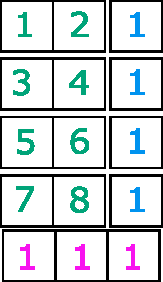
\includegraphics[width=2cm]{Matrix_stack.pdf}
\end{figure}

%%%%%%%%%%%%%%%%%%%%%%%%%%%%%%%%%%%%%%%%%%%%%%%%%%
\newpage
%%%%%%%%%%%%%%%%%%%%%%%%%%%%%%%%%%%%%%%%%%%%%%%%%%
\section*{Lineare Algebra}
\hspace{1cm}
\rowcolors{1}{blue!10}{white}
\begin{tabular}{|l l|}
	\hline
	np.cross(a, b, axisa=-1, axisb=-1, axisc=-1, axis=None) ndarray
	\\np.dot(a, b, out=None) ndarray
	\\np.linalg.det(a) array like
	\\np.linalg.eig(a) ndarray
	\\np.inner(a, b) ndarray
	\\np.linalg.inv(a) ndarray
	\\np.matmul(x1, x2, **kwargs) ndarray
	\\np.linalg.matrix rank(M, tol=None, hermitian=False) array like
	\\np.linalg.norm(x, ord=None, axis=None, keepdims=False) float|ndarray
	\\np.outer(a, b, out=None) ndarray
	\\np.linalg.solve(a, b) ndarray
	\\M @ v ndarray
	\\np.trace(a, offset=0, axis1=0, axis2=1, dtype=None, out=None) ndarray
	
	\\\hline
\end{tabular}
\\
Der @ Operator matmul und dot machen eigentlich das selbe, auf verschieden Arten.\\
trace: die Spur der Matrix.

\vspace{0.5cm}
\begin{minipage}[h]{12cm}
	
	\lstinputlisting{code/Matrix/linalg.py}
\end{minipage}
\begin{minipage}[h]{8cm}
	\textcolor{red}{\textbf{Out:}}
	M4x2= [[0, 1],
	[2, 3],
	[4, 5],
	[6, 7]]
	\\
	= [2,  8, 14, 20 ]
	\\
	
	
\end{minipage}
%%%%%%%%%%%%%%%%%%%%%%%%%%%%%%%%%%%%%%%%%%%%%%%%%%


